\documentclass[10pt]{article}
\usepackage[utf8]{inputenc}
\usepackage{amssymb}
\usepackage{pgf}
\usepackage{tikz,pgfplots}
\pgfplotsset{compat=1.15}
\usepackage[pdftex,
              bookmarks,
              bookmarksnumbered=true,
              bookmarksopen=false,
              colorlinks,
              citecolor=black,
              filecolor=black,
              linkcolor=black,
              urlcolor=black,
              pdfauthor={Alejandro Garces},
              pdftitle={A review of matrix algebra for power and energy applications},
              pdftoolbar=true,
              pdfmenubar=true,
              pdffitwindow = true
              ]{hyperref}
\usepackage{xcolor}

\begin{document}

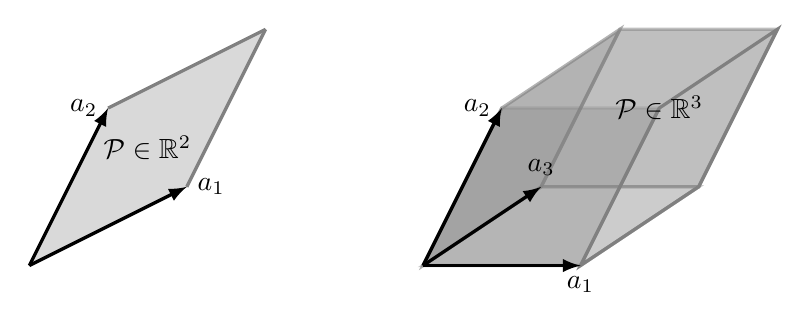
\begin{tikzpicture}[x=1mm,y=1mm]
    \fill[gray!30] (0,0) -- (20,10) -- (30,30) -- (10,20) -- cycle;
    \draw[very thick,gray] (10,20) -- +(20,10);
    \draw[very thick,gray] (20,10) -- +(10,20);
    \draw[-latex,very thick] (0,0) -- (20,10) node[right] {$a_1$};
    \draw[-latex,very thick] (0,0) -- (10,20) node[left] {$a_2$};
    \node at (15,15) {$\mathcal{P}\in\mathbb{R}^2$};
\begin{scope}[shift={(50,0)}]
    \draw[very thick,gray,fill,opacity=0.4] 
    (0,0) -- (15,10) -- (35,10) -- (20,0) -- cycle;
    \draw[very thick,gray,fill,opacity=0.6] 
    (0,0) -- (10,20) -- (25,30) -- (15,10) -- cycle;
    \draw[very thick,gray,fill,opacity=0.5] 
    (15,10) -- (25,30) -- (45,30) -- (35,10) -- cycle;
    \draw[very thick,gray] 
    (20,0) -- (35,10) -- (45,30) -- (30,20) -- cycle;
    \draw[very thick,gray,fill,opacity=0.3] 
    (0,0) -- (20,0) -- (30,20) -- (10,20) -- cycle;

    \draw[-latex,very thick] (0,0) -- (20,0) node[below] {$a_1$};
    \draw[-latex,very thick] (0,0) -- (10,20) node[left] {$a_2$};
    \draw[-latex,very thick] (0,0) -- (15,10) node[above] {$a_3$};
    \node at (30,20) {$\mathcal{P}\in\mathbb{R}^3$};
\end{scope}            
\end{tikzpicture}

\end{document}